% Requirements are LaTeX (e.g. texlive), TikZ, and rubber.
% Build using the following command.
% rubber --pdf full-description


\documentclass{article}

\usepackage{subfig}
\usepackage{tikz}
\usetikzlibrary{arrows,positioning}

\begin{document}

\section{models and parameter values}

This technical note shows some likelihoods and transition expectations
for toy variants of some models, using fixed parameter values.
The evolutionary models consists of jump processes which are continuous in time
and have at least 6 states which are analogous to the 61 codon states
in the universal (non-toy) genetic code.
In the toy genetic code, there are 3 `tolerance classes'
which are analogous to the 20 amino acids in the universal genetic code.

The first variant models changes only among the 6 states.

The second variant is the model of Liwen, Jeff, and Eric,
which considers a special reference state
for which some amino acids are not tolerated.
In the directions on the tree away from the reference node,
a one-way transition from the reference state to the `default'
state is allowed.
The default state allows all amino acids.
In this technical note, the switching rate is fixed at 1.0.
This is the instantaneous rate away from the reference state,
in units of the expected number of primary state changes
in the default state.

The third variant is the blinking model.
In this model, any amino acid may be tolerated or untolerated,
with the restriction that at any given time the amino acid of the current
codon must be tolerated.
In this technical node, the tolerance rates on and off are both fixed at 1.0.
Again, this is in units of the expected number of primary state changes
...


% This rate matrix figure copypasted from ratematrix.tex.
\begin{figure}
\centering
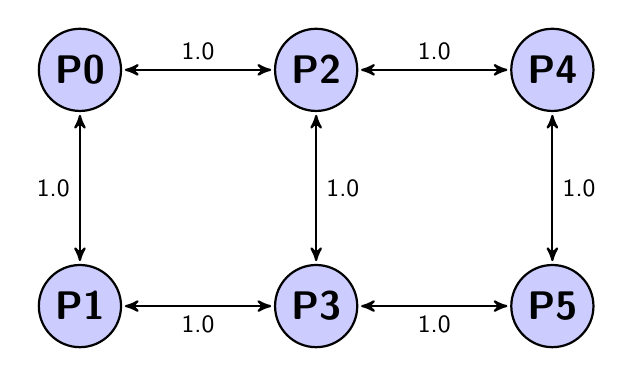
\begin{tikzpicture}[<->,>=stealth',shorten >=1pt,shorten <=1pt,
  auto,node distance=3cm,thick,
  main node/.style={circle,fill=blue!20,draw,font=\sffamily\Large\bfseries}]

  \node[main node] (0) {P0};
  \node[main node] (1) [below of=0] {P1};
  \node[main node] (2) [right of=0] {P2};
  \node[main node] (3) [below of=2] {P3};
  \node[main node] (4) [right of=2] {P4};
  \node[main node] (5) [below of=4] {P5};

  \path[every node/.style={font=\sffamily\small}]
    (0) edge node [left] {1.0} (1)
    (2) edge node [right] {1.0} (3)
    (4) edge node [right] {1.0} (5)
    (0) edge node [above] {1.0} (2)
    (2) edge node [above] {1.0} (4)
    (1) edge node [below] {1.0} (3)
    (3) edge node [below] {1.0} (5);

\end{tikzpicture}
\caption{
	The neutral unscaled substitution rates
	among the primary (codon-like) states
	P0, P1, P2, P3, P4, and P5.
}
\end{figure}

% This simplified codon model figure is from code.tex.
\begin{figure}
\centering
\begin{tabular}{c c}
  primary & tolerance \\
  state & class \\
  \hline
  P0 & T0 \\
  P1 & T0 \\
  P2 & T1 \\
  P3 & T1 \\
  P4 & T2 \\
  P5 & T2
\end{tabular}
\caption{
	Each primary state is associated with a tolerance class.
	In the context of our appliction to molecular biology,
	tolerance classes are analogous to amino acids
	and primary states are analogous to codons.
	In that sense, this table is like a toy genetic code
	with 6 codons instead of 61,
	and with 3 amino acids instead of 20.
}
\end{figure}

% This tree figure is from tree.tex.
\begin{figure}
\centering
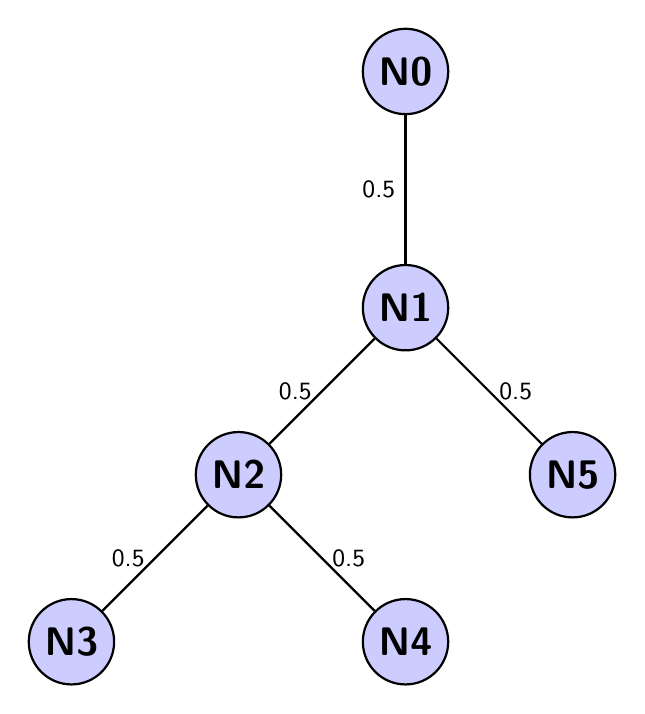
\begin{tikzpicture}[-,>=stealth',auto,node distance=3cm,thick,
  main node/.style={circle,fill=blue!20,draw,font=\sffamily\Large\bfseries}]

  \node[main node] (0) {N0};
  \node[main node] (1) [below of=0] {N1};
  \node[main node] (2) [below left of=1] {N2};
  \node[main node] (3) [below left of=2] {N3};
  \node[main node] (4) [below right of=2] {N4};
  \node[main node] (5) [below right of=1] {N5};

  \path[every node/.style={font=\sffamily\small}]
    (0) edge node [left] {0.5} (1)
    (1) edge node [left] {0.5} (2)
    (2) edge node [left] {0.5} (3)
    (2) edge node [right] {0.5} (4)
    (1) edge node [right] {0.5} (5);

\end{tikzpicture}
\caption{
	This tree will be used for the toy example.
	The branch lengths define the expected number of
	primary state transitions (analogous to codon substitutions)
	when the primary process is unconstrained by selection.
	In general, fewer primary state transitions would be expected
	when selection is at work, for example in the reference process
	(as opposed to the default process) in the irreversible-switch model,
	or when some tolerance classes are in the untolerated state
	in the blinking model.
}
\end{figure}

% This figure merges two figures from data.tex.
\begin{figure}
\centering
\begin{tabular}{c c c c c}
	     & primary &    &    &    \\
	node & state   & T0 & T1 & T2 \\
  \hline
  N0 & P0 & on & (off) & (on) \\
  N1 & ? & ? & ? & ? \\
  N2 & ? & ? & ? & ? \\
  N3 & P4 & ? & ? & on \\
  N4 & P5 & ? & ? & on \\
  N5 & P1 & on & ? & ?
\end{tabular}
\caption{
	This table provides primary state and tolerance state data.
	Some of the nodes have known primary states.
	This is analogous to alignment data for a single codon site.
	For some of the nodes,
	some of the tolerance classes have known states.
	The states enclosed by parentheses represent
	disease data.
}
\end{figure}


\section{pure primary process likelihoods and expectations}

\subsection{no data}
\begin{verbatim}
likelihood: 1.0

edge expectations:
(0, 1) 0.5
(1, 2) 0.5
(2, 3) 0.5
(2, 4) 0.5
(1, 5) 0.5
\end{verbatim}

\subsection{alignment data (primary states) only}
\begin{verbatim}
likelihood: 9.79116182935e-05

edge expectations:
(0, 1) 0.813394611574
(1, 2) 1.75136255298
(2, 3) 0.813394611574
(2, 4) 0.813394611574
(1, 5) 0.813394611574
\end{verbatim}

\section{reference-to-default switching model likelihoods and expectations}

\subsection{no data}
\begin{verbatim}
likelihood: 1.0

synonymous primary state transition edge expectations:
(0, 1) 0.214285714286
(1, 2) 0.214285714286
(2, 3) 0.214285714286
(2, 4) 0.214285714286
(1, 5) 0.214285714286

non-synonymous primary state transition edge expectations:
(0, 1) 0.173294474204
(1, 2) 0.217528223274
(2, 3) 0.244357348279
(2, 4) 0.244357348279
(1, 5) 0.217528223274

reference-to-default edge expectations:
(0, 1) 0.393469340287
(1, 2) 0.238651218541
(2, 3) 0.144749281023
(2, 4) 0.144749281023
(1, 5) 0.238651218541
\end{verbatim}

\subsection{alignment data (primary states) only}
\begin{verbatim}
likelihood: 6.34004488273e-05

synonymous primary state transition edge expectations:
(0, 1) 0.530243839876
(1, 2) 0.214285714286
(2, 3) 0.530243839876
(2, 4) 0.530243839876
(1, 5) 0.530243839876

non-synonymous primary state transition edge expectations:
(0, 1) 0.217796813163
(1, 2) 1.56369681272
(2, 3) 0.308748740396
(2, 4) 0.308748740396
(1, 5) 0.225869938309

reference-to-default edge expectations:
(0, 1) 0.599991615587
(1, 2) 0.255955239807
(2, 3) 0.0579061398365
(2, 4) 0.0579061398365
(1, 5) 0.154937631458
\end{verbatim}

\subsection{alignment data and disease data}
\begin{verbatim}
likelihood: 1.22879715057e-05

synonymous primary state transition edge expectations:
(0, 1) 0.530243839876
(1, 2) 0.214285714286
(2, 3) 0.530243839876
(2, 4) 0.530243839876
(1, 5) 0.530243839876

non-synonymous primary state transition edge expectations:
(0, 1) 0.121658049219
(1, 2) 1.61969296399
(2, 3) 0.329160691143
(2, 4) 0.329160691143
(1, 5) 0.142258701234

reference-to-default edge expectations:
(0, 1) 0.762800997859
(1, 2) 0.236825800216
(2, 3) 0.000373201924736
(2, 4) 0.000373201924736
(1, 5) 0.0873829388166
\end{verbatim}


\section{blinking model likelihoods and expectations}

\subsection{no data}
\begin{verbatim}
likelihood: 1.0

synonymous primary state transition edge expectations:
(0, 1) 0.214285714286
(1, 2) 0.214285714286
(2, 3) 0.214285714286
(2, 4) 0.214285714286
(1, 5) 0.214285714286

non-synonymous primary state transition edge expectations:
(0, 1) 0.142857142857
(1, 2) 0.142857142857
(2, 3) 0.142857142857
(2, 4) 0.142857142857
(1, 5) 0.142857142857

gain-of-tolerance edge expectations:
(0, 1) 0.5
(1, 2) 0.5
(2, 3) 0.5
(2, 4) 0.5
(1, 5) 0.5

loss-of-tolerance edge expectations:
(0, 1) 0.5
(1, 2) 0.5
(2, 3) 0.5
(2, 4) 0.5
(1, 5) 0.5
\end{verbatim}

\subsection{alignment data (primary states) only}
\begin{verbatim}
likelihood: 2.71488210307e-05

synonymous primary state transition edge expectations:
(0, 1) 0.530243839876
(1, 2) 0.214285714286
(2, 3) 0.530243839876
(2, 4) 0.530243839876
(1, 5) 0.530243839876

non-synonymous primary state transition edge expectations:
(0, 1) 0.214361006829
(1, 2) 1.63974144573
(2, 3) 0.214361006829
(2, 4) 0.214361006829
(1, 5) 0.214361006829

gain-of-tolerance edge expectations:
(0, 1) 0.679310052688
(1, 2) 0.540928083993
(2, 3) 0.316402335024
(2, 4) 0.316402335024
(1, 5) 0.316402335024

loss-of-tolerance edge expectations:
(0, 1) 0.316402335024
(1, 2) 0.540928083993
(2, 3) 0.679310052688
(2, 4) 0.679310052688
(1, 5) 0.679310052688
\end{verbatim}

\subsection{alignment data and disease data}
\begin{verbatim}
likelihood: 5.85943537987e-06

synonymous primary state transition edge expectations:
(0, 1) 0.530243839876
(1, 2) 0.214285714286
(2, 3) 0.530243839876
(2, 4) 0.530243839876
(1, 5) 0.530243839876

non-synonymous primary state transition edge expectations:
(0, 1) 0.115905720866
(1, 2) 1.71225589525
(2, 3) 0.22303974637
(2, 4) 0.22303974637
(1, 5) 0.128868804275

gain-of-tolerance edge expectations:
(0, 1) 0.880141827661
(1, 2) 0.563730372337
(2, 3) 0.307552791569
(2, 4) 0.307552791569
(1, 5) 0.315487814895

loss-of-tolerance edge expectations:
(0, 1) 0.30799029452
(1, 2) 0.524525848196
(2, 3) 0.685431320483
(2, 4) 0.685431320483
(1, 5) 0.681655127317
\end{verbatim}



\end{document}




